\documentclass[10pt,a4paper]{article}
\usepackage[utf8]{inputenc}
\usepackage[margin=0.75in]{geometry}
\usepackage{amsmath}
\usepackage{amsfonts}
\usepackage{amssymb}
\usepackage{graphicx}
\usepackage{hyperref}
\author{Chris Mamon}
\title{Angiography + OCT Reconstruction in Python}
\date{}
\begin{document}
	\maketitle
	\section{Package/Environment Managers and Editors}
		Before we dive into the reconstruction we need to set up a python environment and editor. The package and virtual environment manager we have chosen is \textbf{Miniconda} and the editor is \textbf{Visual Studio Code}.
		
		\href{https://docs.conda.io/en/latest/miniconda.html}{Miniconda} is a free minimal installer for \href{https://www.anaconda.com/distribution/}{conda}. We will use it to manage python packages and environments. If you are unfamiliar with these two terms:
		\begin{itemize}
			\item \href{https://realpython.com/python-modules-packages/#reloading-a-module}{Packages}: Are hierarchical structures 	containing python programs.	
			\item \href{https://www.geeksforgeeks.org/python-virtual-environment/}{Virtual Environments}: Isolate python dependencies from ones another, allowing developers to easily separate projects on the same device.
		\end{itemize}
		\begin{figure}[h]
			\centering
			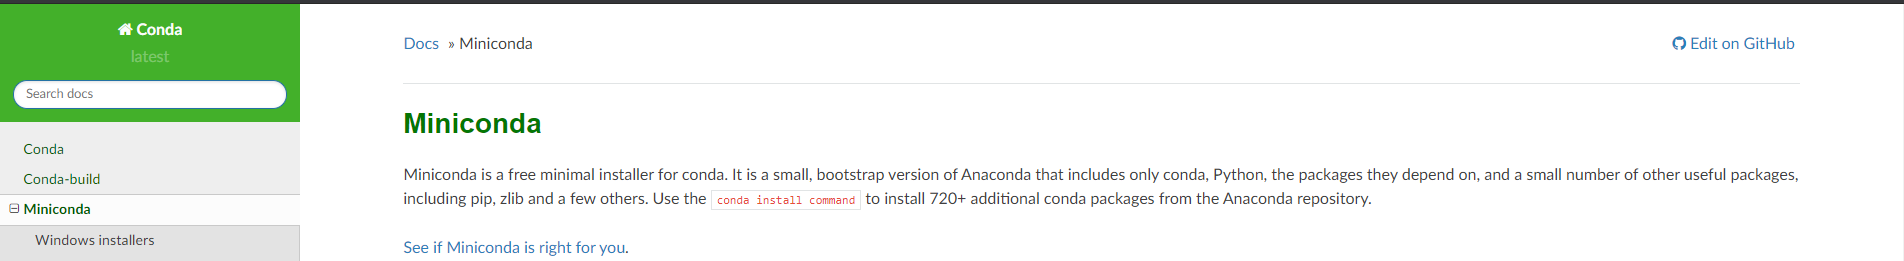
\includegraphics[scale=0.25]{figures/miniconda.PNG}
			\caption{Miniconda download and documentation page \url{https://docs.conda.io/en/latest/miniconda.html}}
		\end{figure}
		
		\href{https://code.visualstudio.com/}{Visual Studio Code} is a source-code editor developed by Microsoft for Windows, Linux and macOS. It includes support for debugging, embedded Git control and GitHub, syntax highlighting, intelligent code completion, snippets, and code refactoring. It is my personal editor of choice due to its light weight nature, high customizability and powerful debugging.
		\begin{figure}[h]
			\centering
			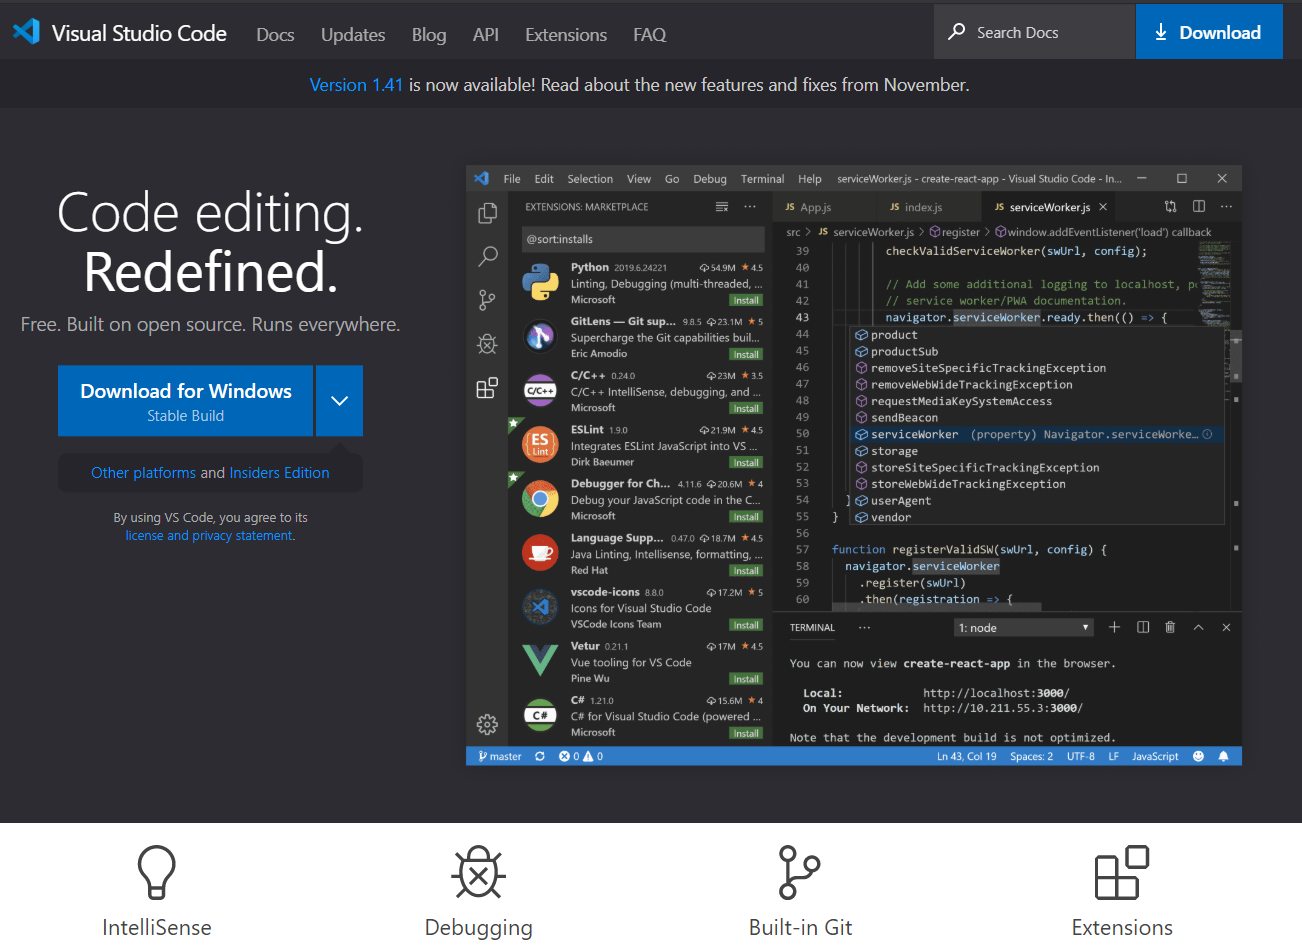
\includegraphics[scale=0.25]{figures/vsc_page.PNG}
			\caption{Visual studio code homepage \url{https://code.visualstudio.com/}}
		\end{figure}
	\section{Github}
		\href{https://github.com/}{Github} is a \href{https://git-scm.com/}{Git} repository hosting service. Git is a distributed version-control system for tracking changes in source code during software development. The \href{https://github.com/hj40/pymethods}{source code} for this project hosted in github and can be downloaded directly 
	\section{Setting up a Miniconda Environment in Visual Studio Code}
		hi
		
		
\end{document}